%
\paragraph{}
In training HMM, we tried on several number of hidden state in our model and chose the numjber of state with the highest emission probabilities as the favorate model in the project. To be specific, we tried on models with 5, 10, 20, 40, 80, 100,and 200. We are working on model with 1000 hidden states because there are around 3000 words in Shakespeare's poetry set and blow 100 words for each group. In our training of Hidden Markov Model,  we maximal the emitting probability of the training set rather than minimizing the Frobenius norm of differeces in \textbf{transition matrix} and \textbf{observation matrix} for the simple reason that in this unsupervised training, the shape of trnasition matrix and observation matrix differs a lot : observation matrix has much more elements than transition matrix in most of the test cases, with number of hidden states 5, 10, and 20, for
instancce. So we maximize the emitting probability instead. Figure \ref{fig:probability} shows when the number of states increases of $\log P$ will increase accordingly. This is to say that choosing number of states according to emitting probability may not be good since if the number of state is too large, say, close to the number of words in each group, the hidden states themselves are not representative.
 \begin{figure}[h!]
 \centering
 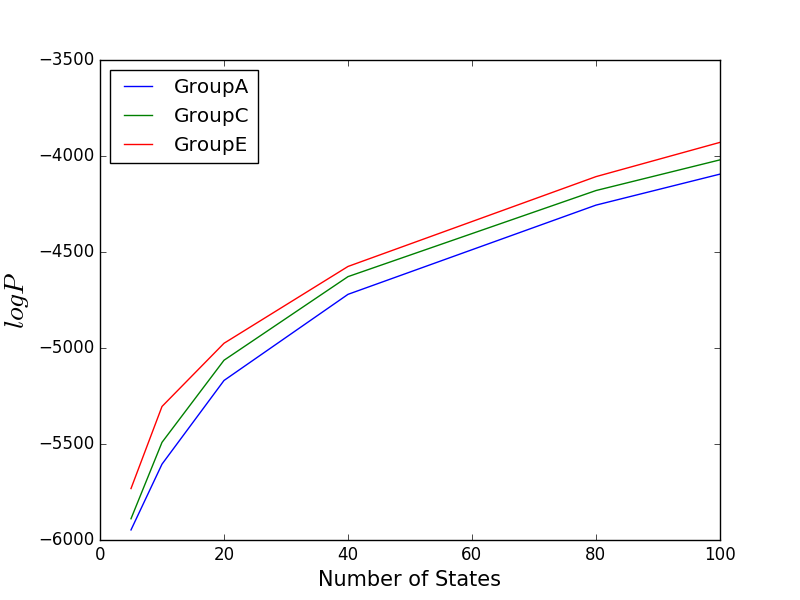
\includegraphics[width=0.6\textwidth]{./figure/probability.png}
 \caption{The emitting probability on training set \textit{Group A}, \textit{Group C} and \textit{Group E} the vertical axis is kept as $\log P$\label{fig:probability}}
 \end{figure}
\paragraph{The Optimal choice for the number of states} Usually, the way to choose the right number of hidden state is to do cross validation: train a model on one part of the corpus (training set) and calculate the emitting probability of the other half of the corpus (testing set) and choose the number that can maximize the emitting probability of the testing set.

\paragraph{}
However, since the fact that most of the words in the corpus appears only once, we abandon the cross validation approach. We choose the best hidden state number by inspecting the quality of the generated sentences. We decide that the larger the number is, the better the generated poem will be. We will elaborate this problem at a later section. 
